\documentclass[a5paper, 10pt]{article}

% Текст
\usepackage[utf8]{inputenc} % UTF-8 кодировка
\usepackage[russian]{babel} % Русский язык
\usepackage{indentfirst} % красная строка в первом параграфе в главе
% Отображение страниц
\usepackage{geometry} % размеры листа и отступов
\usepackage{listings}
\usepackage{color}

\geometry{
	left=12mm,
	top=25mm,
	right=15mm,
	bottom=17mm,
	marginparsep=0mm,
	marginparwidth=0mm,
	headheight=10mm,
	headsep=7mm,
	nofoot}
\usepackage{afterpage,fancyhdr} % настройка колонтитулов
\pagestyle{fancy}
\fancypagestyle{style}{ % создание нового стиля style
	\fancyhf{} % очистка колонтитулов
	\fancyhead[LO, RE]{Лабораторная работа № 5 } % название документа наверху
	\fancyhead[RO, LE]{Спектральная теория графов} % название section наверху
	\fancyfoot[RO, LE]{\thepage} % номер страницы справа внизу на нечетных и слева внизу на четных
	\renewcommand{\headrulewidth}{0.25pt} % толщина линии сверху
	\renewcommand{\footrulewidth}{0pt} % толцина линии снизу
}
\fancypagestyle{plain}{ % создание нового стиля plain -- полностью пустого
	\fancyhf{}
	\renewcommand{\headrulewidth}{0pt}
}
\fancypagestyle{title}{ % создание нового стиля title -- для титульной страницы
	\fancyhf{}
	\fancyhead[C]{{\footnotesize
			Министерство образования и науки Российской Федерации\\
			Федеральное государственное автономное образовательное учреждение высшего образования
	}}
	\fancyfoot[C]{{\large 
			Санкт-Петербург, 2023-2024
	}}
	\renewcommand{\headrulewidth}{0pt}
}

% Математика
\usepackage{amsmath, amsfonts, amssymb, amsthm} % Набор пакетов для математических текстов
%\usepackage{dmvnbase} % мехматовский пакет latex-сокращений
\usepackage{cancel} % зачеркивание для сокращений
% Рисунки и фигуры
\usepackage[pdftex]{graphicx} % вставка рисунков
\usepackage{wrapfig, subcaption} % вставка фигур, обтекая текст
\usepackage{caption} % для настройки подписей
\captionsetup{figurewithin=none,labelsep=period, font={small,it}} % настройка подписей к рисункам
% Рисование
\usepackage{tikz} % рисование
\usepackage{circuitikz}
\usepackage{pgfplots} % графики
% Таблицы
\usepackage{multirow} % объединение строк
\usepackage{multicol} % объединение столбцов
% Остальное
\usepackage[unicode, pdftex]{hyperref} % гиперссылки
\usepackage{enumitem} % нормальное оформление списков
\setlist{itemsep=0.15cm,topsep=0.15cm,parsep=1pt} % настройки списков
% Теоремы, леммы, определения...
\theoremstyle{definition}
\newtheorem{Def}{Определение}
\newtheorem*{Axiom}{Аксиома}
\theoremstyle{plain}
\newtheorem{Th}{Теорема}
\newtheorem{Lem}{Лемма}
\newtheorem{Cor}{Следствие}
\newtheorem{Ex}{Пример}
\theoremstyle{remark}
\newtheorem*{Note}{Замечание}
\newtheorem*{Solution}{Решение}
\newtheorem*{Proof}{Доказательство}
% Свои команды
\newcommand{\comb}[1]{\left[\hspace{-4pt}\begin{array}{l}#1\end{array}\right.\hspace{-5pt} } % совокупность уравнений
% Титульный лист
\usepackage{csvsimple-l3}
\newcommand*{\titlePage}{
	\thispagestyle{title}
	\begingroup
	\begin{center}
		%		{\footnotesize
			%			Министерство образования и науки Российской Федерации\\
			%			Федеральное государственное автономное образовательное учреждение высшего образования
			%		}
		%		
		\vspace*{6ex}
		
		{\small
			САНКТ-ПЕТЕРБУРГСКИЙ НАЦИОНАЛЬНЫЙ ИССЛЕДОВАТЕЛЬСКИЙ УНИВЕРСИТЕТ ИТМО	
		}
		
		\vspace*{2ex}
		
		{\normalsize
			Факультет систем управления и робототехники
		}
		
		\vspace*{15ex}
		
		{\Large \bfseries 
			Лабораторная работа № 5
		}
\vspace*{2ex}
	{\Large \bfseries 
			
"Спектральная теория графов"
		}
\vspace*{2ex}
		
		{\normalsize
			по дисциплине Практическая линейная алгебра
		}

	\end{center}
	\vspace*{20ex}
	\begin{flushright}
		{\large 
			\underline{Выполнила}: студентка гр. \textbf{R3238}\\
			\begin{flushright}
				\textbf{Нечаева А. А.}\\
			\end{flushright}
		}
		
		\vspace*{5ex}
		
		{\large 
			\underline{Преподаватель}: \textit{Перегудин Алексей Алексеевич}
		}
	\end{flushright}	
	\newpage
	\setcounter{page}{1}
	\endgroup}

\begin{document}
	\titlePage
	\pagestyle{style}
\newpage
\section{Кластеризация социальной сети}
Для начала построим модель небольшой социальной сети, где каждый пользователь обозначен одной из 18 вершин графа, а ребра показывают дружбу между людьми.

\begin{figure}[h!]
\center{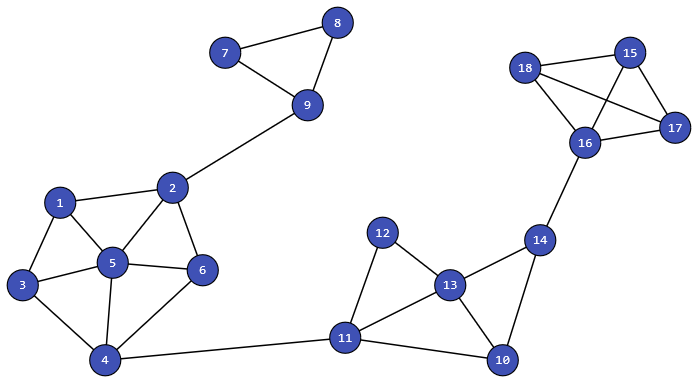
\includegraphics[width=1\linewidth]{pic/1_orig.png}}
\caption{Модель социальной небольшой сети}
\end{figure}
Соотвествующая графу на рисунке 1 матрица Лапласа:
\begin{figure}[h!]
\center{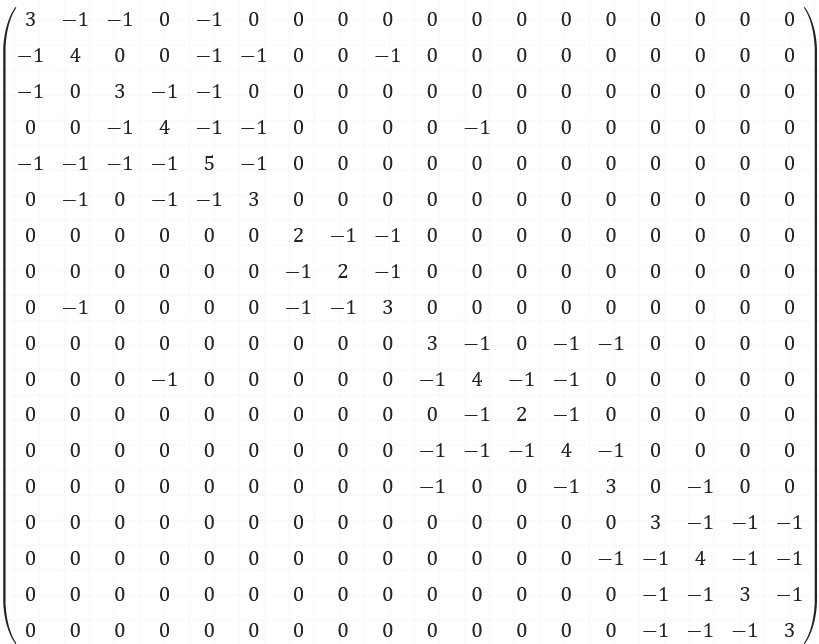
\includegraphics[width=1\linewidth]{pic/lap_1.png}}
\caption{Матрица Лапласа}
\end{figure}
Все собственные числа и соответствующие им собственные векторы приведены в разделе \textit{Приложение} в конце документа.\\

\newpage
\,
\newpage
Выберем $k=4$ компоненты кластеризации графа. И составим матрицу из 4 собственных векторов матрицы Лапласа, соответствующих самым маленьким собственным числам. 

\begin{equation}
V =
\left(\begin{matrix}
1 & -0,541  & -0,569 & 1,766\\
1 & -0,609 & -0,184 & 1,141\\
1 & -0,470 & -0,736 & 1,718\\
1 & -0,329 & -0,803 & 0,976\\
1 & -0,497 & -0,614 & 1,569\\
1 & -0,493 & -0,594 & 1,470\\
1 & -0,933 & 1,570 & -1,573\\
1 & -0,933 & 1,570 & -1,573\\
1 & -0,850 & 1,096 & -0,799\\
1 & 0,375 & -0,885 & -1,742\\
1 & 0,173 & -1,026 & -1,333\\
1 & 0,276 & -1,160 & -2,090\\
1 & 0,355 & -0,944 & -1,819\\
1 & 0,564 & -0,419 & -1,217\\
1 & 1 & 1 & 1\\
1 & 0,911 & 0,698 & 0,508\\
1 & 1 & 1 & 1\\
1 & 1 & 1 & 1
\end{matrix}\right)
\end{equation}
Рассмотрим строки составленной матрицы $V$ как точки пространства  $R^4$. Применим к этим точкам метод  кластеризации $k-means$, реализованный на языке $Python$.
\begin{center}
\begin{lstlisting}
 kmeans = KMeans(n_clusters=4)

    d = np.array([[1, -0.541, -0.569, 1.766],
                  [1, -0.609, -0.184, 1.141],
                  [1, -0.470, -0.736, 1.718],
                  [1, -0.329, -0.803, 0.976],
                  [1, -0.497, -0.614, 1.569],
                  [1, -0.493, -0.594, 1.470],
                  [1, -0.933, 1.570, -1.573],
                  [1, -0.933, 1.570, -1.573],
                  [1, -0.850, 1.096, -0.799],
                  [1, 0.375, -0.885, -1.742],
                  [1, 0.173, -1.026, -1.333],
                  [1, 0.276, -1.160, -2.090],
                  [1, 0.355, -0.944, -1.819],
                  [1, 0.564, -0.419, -1.217],
                  [1, 1, 1, 1],
                  [1, 0.911, 0.698, 0.508],
                  [1, 1, 1, 1],
                  [1, 1, 1, 1]
                  ])
    kmeans.fit(d)
    print(kmeans.labels_)
\end{lstlisting}
\textit{Листинг 1. Фрагмент кода кластеризации.}
\end{center}
В результате выполнения программы получили:
\begin{figure}[h!]
\center{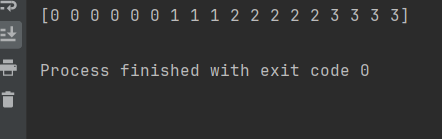
\includegraphics[width=0.5\linewidth]{pic/result.png}}
\caption{Результат кластеризации}
\end{figure}

Соотвествующий вычисленной кластеризации граф изображен на рисунке 4.
\begin{figure}[h!]
\center{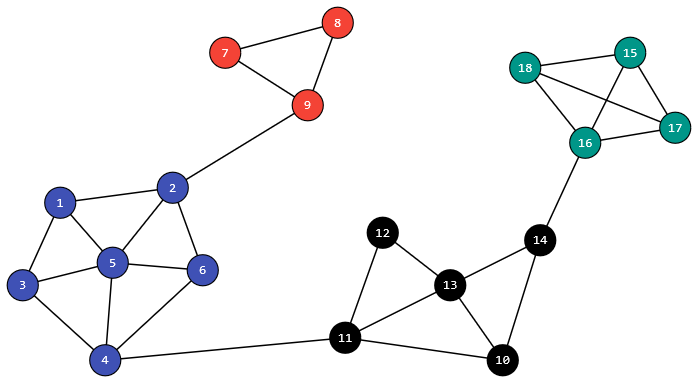
\includegraphics[width=0.7\linewidth]{pic/1_col.png}}
\caption{Граф раскрашенный в соответствии с полученной кластеризацией $k=4$}
\end{figure}
\newpage
Так же проведена кластеризация для значений $k=5$ и $k=6$, результаты представлены на рисунках 5 и 6 соответственно.
\begin{figure}[h!]
\center{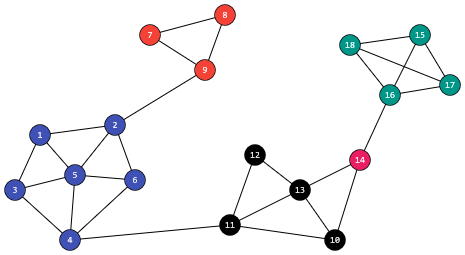
\includegraphics[width=1\linewidth]{pic/5_c.png}}
\caption{Граф раскрашенный в соответствии с полученной кластеризацией $k=5$}
\end{figure}
\begin{figure}[h!]
\center{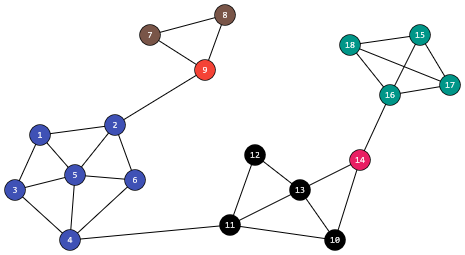
\includegraphics[width=1\linewidth]{pic/6_c.png}}
\caption{Граф раскрашенный в соответствии с полученной кластеризацией $k=6$}
\end{figure}
\\
1. Результат, полученный для кластеризации при $k=4$ иллюстрирует изначально заложенное разделение вершин графа на 4 сообщества.\\
\\2. При $k=5$ глобально остаются те же 4 больших кластера, что и в предыдущем случае, но еще выделяется 1 кластер представленный вершиной номер 14, расположенной как бы на границе двух кластеров. Заметим, что у этой вершины всего 3 связи: 2 связывают с черным кластером, 1 с зеленым, то есть у нее достаточно слабая связь с каждым из больших смежных кластеров. Для сравнения рассмотрим, например, вершину под номером 11 также расположенную на границе крупных кластеров: синего и черного, однако она "крепче" связана с черным кластером, благодаря 3 связям, поэтому не была выделена в отдельный кластер на данном этапе.\\
\\3. При $k=6$ к предыдущему результату добавляется еще 1 кластер, в этот раз представленный вершиной 9 расположенной на границе коричневого и синего кластеров. Заметим, что она так же имеет 3 связи: 2 с коричневым кластером и 1 с синим.\\
\\
\textbf{\textit{4. Почему это работает?}} Вообще, суть кластеризации состоит в группировке элементов множества по какому-то критерию сходства, в данном случае по степени связанности вершин друг с другом. Матрица Лапласа отражает информацию о связях вершин между собой (матрицу смежности) и о количестве вершин, с которыми связана каждая (матрица степеней). Собственные числа матрицы Лапласа всегда вещественные и неотрицательные, их можно отсортировать в порядке неубывания. Наибольший интерес предствляют минимальные из них: например, кратность числа $\lambda = 0$ отражает количество компонент связанности графа, последующие числа -- насколько связи в графе прочны. Метод $k-means$ основывается на поиске центроид (центральных элементов для каждого кластера) и сравнении расстояний от каждого элемента до определенной центроиды. Обратим внимание на матрицу $V$ из собственных векторов (уравнение 1), заметим, что если воспринимать строки матрицы, как некие координаты вершины в пространстве размерности $k$, можно разделить эти точки на $k$ групп, расстояния в которых между каждой парой точек будет минимальным. Поэтому этот довольно успешный метод так распространен в анализе данных.

\newpage
\section{Google PageRank алгоритм}
Придумаемсвязный ориентированный граф из 10 вершин и 25 стрелок (рисунок 7)
\begin{figure}[h!]
\center{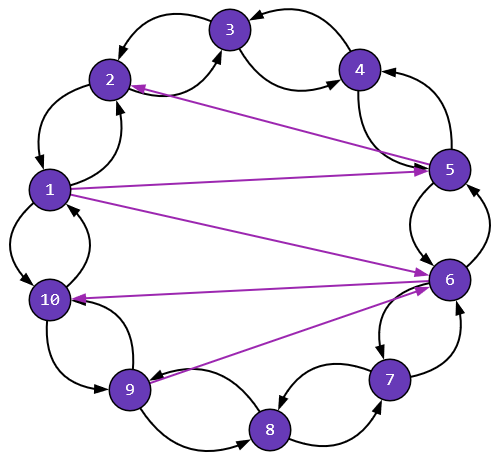
\includegraphics[width=1\linewidth]{pic/g_1.png}}
\caption{Граф связей веб-страниц}
\end{figure}

Составим матрицу 
\begin{equation*}
M=
\begin{pmatrix}
m_{11} & m_{12} & ... & m_{1\,\,\,10}\\
m_{21} & m_{22} & ... & m_{2\,\,\,10}\\
... & ... & ... & ...\\
m_{10\,\,\,1} & m_{10 \,\,\,2} & ... & m_{10\,\,\,10}\\
\end{pmatrix},
\end{equation*}
где $m_{ij}$ -- отношение числа ссылок на $j$-й странице, которые ведут на $i$-ю страницу, к общему числу ссылок на $j$-й странице.
\begin{equation*}
M=
\begin{pmatrix}
0 & 0.5 & 0 & 0 & 0 & 0 & 0 & 0 & 0 & 0.5\\
0.25 & 0 & 0.5 & 0 & \frac{1}{3} & 0 & 0 & 0 & 0 & 0\\
0 & 0.5 & 0 & 0.5 & 0 & 0 & 0 & 0 & 0 & 0\\
0 & 0 & 0.5 & 0 & \frac{1}{3} & 0 & 0 & 0 & 0 & 0\\
0.25 & 0 & 0 & 0.5 & 0 & \frac{1}{3} & 0 & 0 & 0 & 0\\
0.25 & 0 & 0 & 0 & \frac{1}{3} & 0 & 0.5 & 0 & \frac{1}{3} & 0\\
0 & 0 & 0 & 0 & 0 &\frac{1}{3} & 0 & 0.5 & 0 & 0\\
0 & 0 & 0 & 0 & 0 & 0 & 0.5 & 0 & \frac{1}{3} & 0\\
0 & 0 & 0 & 0 & 0 & 0 & 0 & 0.5 & 0 & 0.5\\
0.25 & 0 & 0 & 0 & 0 &  \frac{1}{3} & 0 & 0 & \frac{1}{3} & 0
\end{pmatrix}
\end{equation*}
Собственный вектор матрицы $M$ соответствующий наибольшему собственному числу  $\lambda = 1$:
\begin{equation*}
v = 
\left(\begin{matrix}
\frac{54}{49} \\
\\
\frac{59}{49} \\
\\
\frac{209}{196} \\
\\
\frac{13}{14} \\
\\
\frac{465}{392} \\
\\
\frac{75}{56} \\
\\
\frac{153}{196} \\
\\
\frac{131}{196} \\
\\
\frac{327}{392} \\
\\
1
\end{matrix}\right)
\approx
\left(\begin{matrix}
1.1020 \\
1.2041 \\
1.0663 \\
0.9286 \\
1.1862 \\
1.3393 \\
0.7806 \\
0.6684 \\
0.8342 \\
1
\end{matrix}\right)
\end{equation*}
Ранжируем веб-страницы (вершины графа) в соответствии с \textit{PageRank}-алгоритм при отсутствии затухания ($d = 1$).

\begin{figure}[h!]
\center{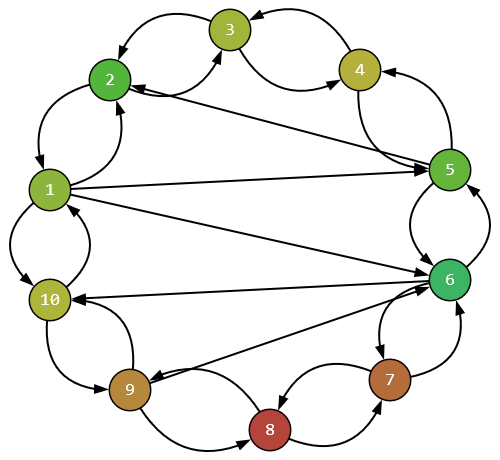
\includegraphics[width=1\linewidth]{pic/g_c.png}}
\caption{Граф ранжированных веб-страниц}
\end{figure}
\newpage
 Рисунок 8 иллюстрирует полученный результат: ярко-зеленый -- самый высокий приоритет, красный -- самый низкий. Соотвествующий список вершин:
\begin{equation*}
\begin{matrix}
1. & 6 & \,\,\,\,\,\, & 6. & 10\\
2. & 2  & \,\,\,\,\,\, & 7. & 4\\
3. & 5  & \,\,\,\,\,\, & 8. & 9\\
4. & 1  & \,\,\,\,\,\, & 9. & 7\\
5. & 3  & \,\,\,\,\,\, &10. & 8
\end{matrix}
\end{equation*}
\\
\textbf{\textit{Почему это работает?}}






\section{Приложение}
Все собственные числа соответствующие им собственные векторы для матрицы Лапласа из задания 1.
\begin{equation*}
\left(\begin{matrix}
1 \\
1 \\
1 \\
1 \\
1 \\
1 \\
1 \\
1 \\
1 \\
1 \\
1 \\
1 \\
1 \\
1 \\
1 \\
1 \\
1 \\
1
\end{matrix}\right)
 , \, \lambda_ 1 = 0\,\,\,\,\,\,\,\,\,\,
\left(\begin{matrix}
0 \\
0 \\
0 \\
0 \\
0 \\
0 \\
-1 \\
1 \\
0 \\
0 \\
0 \\
0 \\
0 \\
0 \\
0 \\
0 \\
0 \\
0
\end{matrix}\right)
, \, \lambda_ 2 = 3\,\,\,\,\,\,\,\,\,\,
\left(\begin{matrix}
0 \\
0 \\
0 \\
0 \\
0 \\
0 \\
0 \\
0 \\
0 \\
0 \\
0 \\
0 \\
0 \\
0 \\
-1 \\
0 \\
1 \\
0
\end{matrix}\right)
, \, \lambda_ 3 = 4\,\,\,\,\,\,\,\,\,\,
\left(\begin{matrix}
0 \\
0 \\
0 \\
0 \\
0 \\
0 \\
0 \\
0 \\
0 \\
0 \\
0 \\
0 \\
0 \\
0 \\
-1 \\
0 \\
1 \\
0
\end{matrix}\right)
, \, \lambda_ 4 = 4\,\,\,\,\,\,\,\,\,\,
\end{equation*}

\begin{equation*}
\left(\begin{matrix}
\left(-0,541\right) \\
\left(-0,609\right) \\
\left(-0,470\right) \\
\left(-0,329\right) \\
\left(-0,497\right) \\
\left(-0,493\right) \\
\left(-0,933\right) \\
\left(-0,933\right) \\
\left(-0,850\right) \\
\left(0,375\right) \\
\left(0,173\right) \\
\left(0,276\right) \\
\left(0,355\right) \\
\left(0,564\right) \\
1 \\
\left(0,911\right) \\
1 \\
1
\end{matrix}\right)
,  \lambda_ 5 = 0.089\,\,\,\,\,\,\,\,\,\,
\left(\begin{matrix}
\left(-0,569\right) \\
\left(-0,184\right) \\
\left(-0,736\right) \\
\left(-0,803\right) \\
\left(-0,614\right) \\
\left(-0,594\right) \\
\left(1,570\right) \\
\left(1,570\right) \\
\left(1,096\right) \\
\left(-0,885\right) \\
\left(-1,026\right) \\
\left(-1,160\right) \\
\left(-0,944\right) \\
\left(-0,419\right) \\
1 \\
\left(0,698\right) \\
1 \\
1
\end{matrix}\right)
,  \lambda_ 6 = 0.302\,\,\,\,\,\,\,\,\,\,
\left(\begin{matrix}
\left(1,766\right) \\
\left(1,141\right) \\
\left(1,718\right) \\
\left(0,976\right) \\
\left(1,569\right) \\
\left(1,470\right) \\
\left(-1,573\right) \\
\left(-1,573\right) \\
\left(-0,799\right) \\
\left(-1,742\right) \\
\left(-1,333\right) \\
\left(-2,090\right) \\
\left(-1,819\right) \\
\left(-1,217\right) \\
1 \\
\left(0,508\right) \\
1 \\
1
\end{matrix}\right)
,  \lambda_ 7 = 0.492\,\,\,\,\,\,\,\,\,\,
\end{equation*}

\begin{equation*}
\left(\begin{matrix}
\left(-0,483\right) \\
\left(-0,304\right) \\
\left(-0,109\right) \\
\left(0,480\right) \\
\left(-0,117\right) \\
\left(0,055\right) \\
\left(0,102\right) \\
\left(0,102\right) \\
\left(-0,092\right) \\
\left(-3,902\right) \\
\left(1,177\right) \\
\left(6,448\right) \\
\left(-0,559\right) \\
\left(-4,895\right) \\
1 \\
\left(-0,904\right) \\
1 \\
1
\end{matrix}\right)
,  \lambda_ 8 = 1.904\,\,\,\,\,\,\,
\left(\begin{matrix}
\left(-112,670\right) \\
\left(51,599\right) \\
\left(-122,421\right) \\
\left(36,220\right) \\
\left(5,800\right) \\
\left(162,222\right) \\
\left(-18,290\right) \\
\left(-18,290\right) \\
\left(26,025\right) \\
\left(2,964\right) \\
\left(11,522\right) \\
\left(-16,445\right) \\
\left(-4,567\right) \\
\left(-5,244\right) \\
1 \\
\left(-1,423\right) \\
1 \\
1
\end{matrix}\right)
,  \lambda_ 9 = 2.423\,\,\,\,\,\,\,\,
\left(\begin{matrix}
\left(-15,810\right) \\
\left(-19,115\right) \\
\left(13,664\right) \\
\left(19,505\right) \\
\left(0,545\right) \\
\left(3,014\right) \\
\left(7,572\right) \\
\left(7,572\right) \\
\left(-12,795\right) \\
\left(2,437\right) \\
\left(8,335\right) \\
\left(-8,656\right) \\
\left(-2,365\right) \\
\left(-5,214\right) \\
1 \\
\left(-1,690\right) \\
1 \\
1
\end{matrix}\right),  \lambda_ {10} =2.690\,\,\,\,\,\,\,\,\,\,
\end{equation*}

\begin{equation*}
\left(\begin{matrix}
\left(0,661\right) \\
\left(0,984\right) \\
\left(-0,783\right) \\
\left(0,071\right) \\
\left(-0,445\right) \\
\left(-1,660\right) \\
\left(-0,872\right) \\
\left(-0,872\right) \\
\left(2,065\right) \\
\left(3,889\right) \\
\left(2,932\right) \\
\left(-2,241\right) \\
\left(0,133\right) \\
\left(-4,497\right) \\
1 \\
\left(-2,368\right) \\
1 \\
1
\end{matrix}\right)
,  \lambda_ {11} =3.368\,\,\,\,\,\,\,\,
\left(\begin{matrix}
\left(9,817\right) \\
\left(-0,245\right) \\
\left(-8,229\right) \\
\left(-5,286\right) \\
\left(1,399\right) \\
\left(5,733\right) \\
\left(6,255\right) \\
\left(6,255\right) \\
\left(-17,018\right) \\
\left(4,618\right) \\
\left(-0,381\right) \\
\left(-0,251\right) \\
\left(0,812\right) \\
\left(-3,760\right) \\
1 \\
\left(-2,721\right) \\
1 \\
1
\end{matrix}\right)
,  \lambda_ {12} =3.721\,\,\,\,\,\,\,
\left(\begin{matrix}
\left(-3,665\right) \\
\left(-0,297\right) \\
\left(5,560\right) \\
\left(-4,796\right) \\
\left(0,190\right) \\
\left(3,295\right) \\
\left(-0,093\right) \\
\left(-0,093\right) \\
\left(0,324\right) \\
\left(5,299\right) \\
\left(-6,706\right) \\
\left(2,647\right) \\
\left(0,121\right) \\
\left(-1,299\right) \\
1 \\
\left(-3,488\right) \\
1 \\
1
\end{matrix}\right)
,  \lambda_ {13} =4.488\,\,\,\,\,\,\,\,\,\,
\end{equation*}

\begin{equation*}
\left(\begin{matrix}
\left(-0,288\right) \\
\left(0,067\right) \\
\left(0,517\right) \\
\left(-0,629\right) \\
\left(-0,047\right) \\
\left(0,327\right) \\
\left(0,013\right) \\
\left(0,013\right) \\
\left(-0,050\right) \\
\left(-3,826\right) \\
\left(-0,251\right) \\
\left(-2,370\right) \\
\left(7,043\right) \\
\left(0,348\right) \\
1 \\
\left(-3,866\right) \\
1 \\
1
\end{matrix}\right)
,  \lambda_ {14} =4.866\,\,\,\,\,\,\,\,\,\,
\left(\begin{matrix}
\left(1,758\right) \\
\left(-2,275\right) \\
\left(-1,818\right) \\
\left(2,390\right) \\
\left(0,041\right) \\
\left(-0,068\right) \\
\left(-0,287\right) \\
\left(-0,287\right) \\
\left(1,236\right) \\
\left(0,292\right) \\
\left(-1,273\right) \\
\left(0,995\right) \\
\left(-2,016\right) \\
\left(2,616\right) \\
1 \\
\left(-4,305\right) \\
1 \\
1
\end{matrix}\right)
,  \lambda_ {15} = 5.305\,\,\,\,\,\,\,\,\,\,
\left(\begin{matrix}
\left(-6,448\right) \\
\left(10,339\right) \\
\left(-0,417\right) \\
\left(2,122\right) \\
\left(5,312\right) \\
\left(-7,523\right) \\
\left(1,245\right) \\
\left(1,245\right) \\
\left(-5,430\right) \\
\left(-0,064\right) \\
\left(-0,263\right) \\
\left(0,831\right) \\
\left(-2,531\right) \\
\left(2,945\right) \\
1 \\
\left(-4,363\right) \\
1 \\
1
\end{matrix}\right)
,  \lambda_ {16} = 5.363\,\,\,\,\,\,\,\,\,\,
\end{equation*}

\begin{equation*}
\left(\begin{matrix}
\left(-0,141\right) \\
\left(2,993\right) \\
\left(5,426\right) \\
\left(-6,661\right) \\
\left(-8,035\right) \\
\left(4,280\right) \\
\left(0,273\right) \\
\left(0,273\right) \\
\left(-1,295\right) \\
\left(-3,217\right) \\
\left(9,878\right) \\
\left(-0,961\right) \\
\left(-6,291\right) \\
\left(5,209\right) \\
1 \\
\left(-4,734\right) \\
1 \\
1
\end{matrix}\right)
,  \lambda_ {17} = 5.734\,\,\,\,\,\,\,\,\,\,
\left(\begin{matrix}
\left(-13,211\right) \\
\left(-42,779\right) \\
\left(-7,706\right) \\
\left(-55,201\right) \\
\left(93,510\right) \\
\left(1,373\right) \\
\left(-2,829\right) \\
\left(-2,829\right) \\
\left(14,873\right) \\
\left(-10,039\right) \\
\left(37,402\right) \\
\left(-5,598\right) \\
\left(-13,572\right) \\
\left(8,864\right) \\
1 \\
\left(-5,257\right) \\
1 \\
1
\end{matrix}\right)
,  \lambda_ {18} = 6.257\,\,\,\,\,\,\,\,\,\,
\end{equation*}

\end{document}













